\documentclass{beamer}

\mode<presentation>
{
  %\usetheme{CambridgeUS}
  %\usetheme{Frankfurt}
  \usetheme{Singapore}
  %\usecolortheme{crane}
  \usefonttheme{professionalfonts}
  %\usefonttheme[onlymath]{serif}
  
  \setbeamertemplate{blocks}[rounded][shadow=true]
}

\usepackage{pgfpages}

\usepackage{alltt,verbatim,amsmath,times,empheq}
\usepackage{bm}
\usepackage[english]{babel}
\usepackage[utf8]{inputenc}

%\usepackage{times}
%\usepackage[T1]{fontenc}
% Or whatever. Note that the encoding and the font should match. If T1
% does not look nice, try deleting the line with the fontenc.

%\usepackage{hyperref}

\usepackage{multimedia,xmpmulti}

\usepackage{animate}

\definecolor{dark red}{HTML}{E41A1C}
\definecolor{dark green}{HTML}{4DAF4A}
\definecolor{dark violet}{HTML}{984EA3}
\definecolor{dark blue}{HTML}{084594}
\definecolor{dark orange}{HTML}{FF7F00}
\definecolor{light blue}{HTML}{377EB8}
\definecolor{light red}{HTML}{FB9A99}
\definecolor{light violet}{HTML}{CAB2D6}

\setbeamercolor{boxed}{fg=black,bg=uaf yellow}

\newcommand{\CC}{\mathbb{C}}
\newcommand{\NN}{\mathbb{N}}
\newcommand{\RR}{\mathbb{R}}
\newcommand{\ZZ}{\mathbb{Z}}
\newcommand{\Acal}{\mathcal{A}}
\newcommand{\Bcal}{\mathcal{B}}
\newcommand{\Ccal}{\mathcal{C}}
\newcommand{\Ncal}{\mathcal{N}}
\newcommand{\Kcal}{\mathcal{K}}

\newcommand{\bF}{\mathbf{F}}
\newcommand{\bQ}{\mathbf{Q}}
\newcommand{\bU}{\mathbf{U}}
\newcommand{\bbU}{\bar{\bU}}
\newcommand{\bu}{\mathbf{u}}
\newcommand{\bv}{\mathbf{v}}
\newcommand{\bx}{\mathbf{x}}

\newcommand{\Div}{\nabla\cdot}
\newcommand{\eps}{\epsilon}
\newcommand{\grad}{\nabla}
\newcommand{\lap}{\triangle}
\DeclareMathOperator{\trace}{tr}
\renewcommand{\bar}{\overline}

\newcommand{\ddx}[1]{\frac{\partial #1}{\partial x}}
\newcommand{\ddy}[1]{\frac{\partial #1}{\partial y}}
\newcommand{\pp}[2]{\frac{\partial #1}{\partial #2}}
\newcommand{\ppt}[1]{\frac{\partial #1}{\partial t}}
\newcommand{\ppT}[1]{\frac{\partial #1}{\partial T}}
\newcommand{\ppx}[1]{\frac{\partial #1}{\partial x}}
\newcommand{\ppy}[1]{\frac{\partial #1}{\partial y}}
\newcommand{\ppz}[1]{\frac{\partial #1}{\partial z}}
\newcommand{\ppxx}[1]{\frac{\partial^2 #1}{\partial x^2}}
\newcommand{\ppzz}[1]{\frac{\partial^2 #1}{\partial z^2}}

\newcommand{\Tnorm}[1]{\left|\!\left|\!\left|#1\right|\!\right|\!\right|}
\newcommand{\rhow}{\rho_{\text{w}}}
\newcommand{\Wq}{W^{1,q}(\Omega)}
\newcommand{\half}{\frac12}

%\setbeamercolor{redtext}{fg=red!80!black}
\setbeamercolor{redtext}{fg=red!94!black}
%\setbeamercolor{greentext}{fg=green!80!black}
\setbeamercolor{greentext}{fg=green!60!black}
%\setbeamercolor{bluetext}{fg=blue!70!black}
\setbeamercolor{bluetext}{fg=blue!90!black}
\setbeamercolor{yellowtext}{fg=yellow!95!black}
\setbeamercolor{orangetext}{fg=yellow!50!red}

\newcommand{\green}{\usebeamercolor[fg]{greentext}}
\newcommand{\blue}{\usebeamercolor[fg]{bluetext}}
\newcommand{\red}{\usebeamercolor[fg]{redtext}}

\renewcommand{\L}{\emph{Left}}
\newcommand{\R}{\emph{Right}}


% this slide reappears so it is a 4/5 argument function
\newcommand{\whatvi}[4]{\longwhatvi{#1}{#2}{#3}{#4}{}}
\newcommand{\longwhatvi}[5]{
\begin{frame}
  \frametitle{what is a \emph{variational inequality}?}

\begin{enumerate}
#1{\item a cute way to rewrite a calc problem in $\RR^1$; min $f$ solves:
   $$u: \qquad f'(u) (v - u) \ge 0 \qquad \text{ for all } v \in [a,b]$$}
\vspace{-4mm}
#2{\item a dot-product for projection on a closed, convex $K\subset \mathcal{H}$:
   $$y=\Pi x: \qquad (y - x) \cdot (\eta - y) \ge 0 \,\, \text{ for all } \eta \in K$$}
\vspace{-4mm}
#3{\item a rewriting of ``min $f$ on convex $K\subset \RR^n$'':
   $$u: \qquad \grad f (u) \cdot (v - u) \ge 0 \qquad \text{ for all } v \in K$$}
\vspace{-4mm}
#4{\item a way to get existence for \emph{any} continuous nonlinear eqns

on compact, convex $K_0\subset \RR^n$:
   $$u: \qquad F(u) \cdot (v - u) \ge 0 \qquad \text{ for all } v \in K_0$$}
\vspace{-4mm}
#5
\end{enumerate}
\end{frame}
}


\title[what is \dots a variational inequality]{What is \dots a \emph{variational inequality}?}

\author[Bueler]{Ed Bueler}

\institute[UAF]{
  \tiny Dept of Mathematics and Statistics and Geophysical Institute \\

  University of Alaska Fairbanks
}

\date{\tiny 30 January, 2014}


\setbeamerfont{date}{size=\scriptsize}

\subject{variational inequality}


%\begin{comment}
\AtBeginSection[]
{
  \begin{frame}<beamer>
    \frametitle{Outline}
    \tableofcontents[currentsection,hideallsubsections]
  \end{frame}
}
%\end{comment}


\begin{document}
\graphicspath{{../commonfigs/}}

\begin{frame}
  \titlepage
\end{frame}


% NO OUTLINE BECAUSE ONE APPEARS AT START OF EACH SECTION:
%\begin{comment}
%\begin{frame}
%  \frametitle{Outline}
%  \tableofcontents[hideallsubsections]
%  % You might wish to add the option [pausesections]
%\end{frame}
%\end{comment}


\begin{frame}
  \frametitle{what is \dots \,the source of my title?}

\begin{center}

\includegraphics[height=0.205\textheight]{what-is-grobner}


\includegraphics[height=0.2\textheight]{what-is-quasimorphism}


\includegraphics[height=0.2\textheight]{what-is-random-matrix}


\includegraphics[height=0.195\textheight]{what-is-systole}
\end{center}
\end{frame}


\section[problems]{problems you can write as variational inequalities}

\begin{frame}
  \frametitle{calculus I problem}

\begin{center}
\includegraphics<1>[height=0.5\textheight]{calcprob_bare.png}
\includegraphics<2>[height=0.5\textheight]{calcprob_soln.png}
\end{center}

\begin{itemize}
\item suppose you have a smooth function \uncover<2>{\emph{on a closed, bounded interval }}
\item and you want to minimize it
\end{itemize}

\end{frame}


\begin{frame}
  \frametitle{calculus I problem}

\begin{center}
\includegraphics[width=0.33\textwidth]{calcprob_soln_interior.png}
\includegraphics[width=0.33\textwidth]{calcprob_soln_leftendpoint.png}
\includegraphics[width=0.33\textwidth]{calcprob_soln_rightendpoint.png}
\end{center}

\vspace{8mm}

because $f$ is smooth, you can say about the minimizer $u$ that:
\only<1>{
\vspace{1mm}

\begin{itemize}
\item if $a < u < b$ then $f'(u)=0$ \emph{or}
\item if $u = a$ then $f'(u) \ge 0$ \emph{or}
\item if $u = b$ then $f'(u) \le 0$
\end{itemize}
}
\only<2>{

the \alert{variational inequality} applies,
    $$f'(u) (v - u) \ge 0 \qquad \text{ for all } v \in [a,b]$$
}
\end{frame}

% where we stand
\longwhatvi{\visible}{\invisible}{\invisible}{\invisible}{\uncover<2>{\vspace{-1cm}\\\centerline{the above is a \emph{necessary condition} only}}}


\begin{frame}
  \frametitle{projection onto a closed, convex set $K \subset \mathcal{H}$}

\begin{center}
\includegraphics[height=0.4\textheight]{proj_xy.png}
\end{center}

\vspace{-4mm}
Suppose $K \subset \RR^n$ is closed and convex.

(Or $K \subset \mathcal{H}$ closed and convex, where $\mathcal{H}$ is a Hilbert space.)

\bigskip

Definition.  Given $x\in\RR^n$ (or $x \in \mathcal{H}$), the unique minimizer
    $$y = \min_{z\in K} \|x-z\|$$
is the \emph{projection} of $x$ onto $K$, written $y = \Pi x$.
\end{frame}


\begin{frame}
  \frametitle{projection onto a closed, convex set $K \subset \mathcal{H}$}

\begin{center}
\includegraphics<1>[height=0.4\textheight]{proj_xy_vect.png}
\includegraphics<2>[height=0.4\textheight]{proj_xyprime_vect.png}
\end{center}

Theorem.
   $$y = \Pi x \qquad \iff \qquad (y - x) \cdot (\eta - y) \ge 0 \,\, \text{ for all } \eta \in K$$

\medskip
This is also a \alert{variational inequality}.

\medskip
\emph{Idea}.  The angle between $y-x$ and $\eta - y$ is $\le 90^\circ$ for all $\eta \in K$.
\end{frame}


% where we stand
\whatvi{\visible}{\visible}{\invisible}{\invisible}


\begin{frame}
  \frametitle{minimize $f$ on convex $K\subset \RR^n$}

\begin{columns}
\begin{column}{0.7\textwidth}
Consider a mainstream math problem:
\begin{itemize}
\item let $K \subset \RR^n$ be convex
\item let $f: \RR^n \to \RR$ be smooth ($C^1$)
\item find $u\in K$ so that $f$ is minimum?
\end{itemize}

\bigskip
\uncover<2->{Claim: if $u\in K$ minimizes $f$ then $u$ solves
   $$\grad f(u)\cdot (v-u) \ge 0 \qquad \text{ for all } v \in K$$}
\uncover<2->{which is a \alert{variational inequality}}
\end{column}
\begin{column}{0.3\textwidth}
\includegraphics<1->[width=1.0\textwidth]{constrained-opt}
\end{column}
\end{columns}
\end{frame}

\begin{frame}
  \frametitle{minimize $f$ on convex $K\subset \RR^n$}

\emph{Theorem}.  $K\subset \RR^n$ convex.  $f:\RR^n\to\RR$ smooth.

\noindent If $u\in K$ minimizes $f$ then
   $$\grad f(u)\cdot (v-u) \ge 0 \qquad \text{ for all } v \in K.$$

\emph{Proof}.  If $0\le t\le 1$ then
    $$(1-t) u + t v\in K$$
But $t=0$ is minimizer of
    $$g(t) = f\left((1-t) u + t v\right)$$
so by the ``calculus I problem'', $g'(0) \ge 0$.  By chain rule
    $$g'(t) = (\grad f)((1-t) u + t v) \cdot (-u + v)$$
so $g'(0) = (\grad f)(u) \cdot (v-u) \ge 0$. \qed
\end{frame}


\begin{frame}
  \frametitle{minimize $f$ on convex $K\subset \RR^n$}

\begin{columns}
\begin{column}{0.7\textwidth}
How about existence of $u$?

It happens if either:
\begin{itemize}
\item $K$ is compact
\item $K$ is closed and $f$ is coercive
\end{itemize}

\bigskip
\bigskip

How about uniqueness of $u$?

It happens if:
\begin{itemize}
\item $f$ is strictly convex
\end{itemize}
\end{column}
\begin{column}{0.3\textwidth}
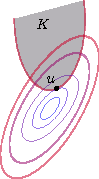
\includegraphics[width=1.0\textwidth]{constrained-opt}
\end{column}
\end{columns}
\end{frame}

% where we stand
\whatvi{\visible}{\visible}{\visible}{\invisible}


\begin{frame}
  \frametitle{FIXME: solve $F(u)=0$ on compact, convex $K_0\subset \RR^n$}

\end{frame}

% where we stand
\whatvi{\visible}{\visible}{\visible}{\visible}


\section[obstacle]{obstacle problem example}

\begin{frame}
  \frametitle{functional and convex set}

$$J[v] = \int_0^L \frac{1}{2} (v')^2 - f v$$

$$\mathcal{K} = \left\{v \in H_0^1 \,:\, v \ge \psi\right\}$$
\end{frame}


\begin{frame}
  \frametitle{convexity}

if $u\in \mathcal{K}$ is minimizer and if $v\in\mathcal{K}$ and if $0\le \eps \le 1$ then

$(1 - \eps) u + \eps v = u + \eps (v-u) \in \mathcal{K}$ because $\mathcal{K}$ is convex 

\vspace{0.5in}

FIXME: picture first as linear combination $(1 - \eps) u + \eps v$

\vspace{0.5in}

FIXME: ... then as vector directed from base: $u + \eps (v-u)$
\end{frame}


\begin{frame}
  \frametitle{first variation calculation}

if $u\in \mathcal{K}$ is minimizer and if $v\in\mathcal{K}$ and if $0\le \eps \le 1$ then
   \begin{align*}
   0 &\le J[u + \eps(v-u)] - J[u] \\
     &= \int_0^L \frac{1}{2} \left[(u'+\eps (v-u)')^2-(u')^2\right] - f \left(u+\eps(v-u) - u\right) \\
     &= \int_0^L \frac{1}{2} \left[(u')^2+ 2 \eps u' (v'-u') + \eps^2 (v'-u')^2 - (u')^2\right] - f \eps(v-u) \\
     &= \eps \int_0^L u' (v'-u') - f (v-u) + \eps^2 \int_0^L (v'-u')^2
   \end{align*}
\end{frame}


\begin{frame}
  \frametitle{whence the variational inequality}

\begin{itemize}
\item so far: if $0<\eps\le 1$
\begin{align*}
0 &\le \frac{J[u + \eps(v-u)] - J[u]}{\eps} \\
  &= \int_0^L u' (v'-u') - f (v-u) + \eps \int_0^L (v'-u')^2
\end{align*}
\item \emph{thus} as $\eps \to 0$, we know that $u\in\mathcal{K}$ satisfies
  $$\int_0^L u' (v'-u') - f (v-u) \ge 0 \qquad \forall v\in\mathcal{K}$$
which is a \alert{variational inequality}
\end{itemize}
\end{frame}


\begin{frame}
  \frametitle{FIXME}

\end{frame}


\begin{frame}
  \frametitle{the 3-point case of obstacle problem}

\begin{columns}
\begin{column}{0.5\textwidth}
\begin{center}
\includegraphics<1>[height=0.5\textheight]{case_f0_psi1_oneD.png}
\includegraphics<2>[height=0.5\textheight]{case_f2_psi0_oneD.png}
\includegraphics<3>[height=0.5\textheight]{case_f2_psi3_oneD.png}
\includegraphics<4>[height=0.5\textheight]{case_f-1_psi-1_oneD.png}
\end{center}
\end{column}
\begin{column}{0.5\textwidth}
\begin{center}
\includegraphics<1>[height=0.5\textheight]{case_f0_psi1_3D.png}
\includegraphics<2>[height=0.5\textheight]{case_f2_psi0_3D.png}
\includegraphics<3>[height=0.5\textheight]{case_f2_psi3_3D.png}
\includegraphics<4>[height=0.5\textheight]{case_f-1_psi-1_3D.png}
\end{center}
\end{column}
\end{columns}

\begin{center}
\only<1>{\framebox[7mm]{1}}
\only<2>{\framebox[7mm]{2}}
\only<3>{\framebox[7mm]{3}}
\only<4>{\framebox[7mm]{4}}
\end{center}
\end{frame}


\begin{frame}
  \frametitle{the 3-point case of obstacle problem, reconsidered}

\begin{columns}
\begin{column}{0.5\textwidth}
\begin{center}
\includegraphics<1>[height=0.5\textheight]{case_f0_psi1_oneD.png}
\includegraphics<2>[height=0.5\textheight]{case_f2_psi0_oneD.png}
\includegraphics<3>[height=0.5\textheight]{case_f2_psi3_oneD.png}
\includegraphics<4>[height=0.5\textheight]{case_f-1_psi-1_oneD.png}
\end{center}
\end{column}
\begin{column}{0.5\textwidth}
\begin{center}
\includegraphics<1>[height=0.5\textheight]{case_f0_psi1_convex.png}
\includegraphics<2>[height=0.5\textheight]{case_f2_psi0_convex.png}
\includegraphics<3>[height=0.5\textheight]{case_f2_psi3_convex.png}
\includegraphics<4>[height=0.5\textheight]{case_f-1_psi-1_convex.png}
\end{center}
\end{column}
\end{columns}

\begin{center}
\only<1>{\framebox[7mm]{1}}
\only<2>{\framebox[7mm]{2}}
\only<3>{\framebox[7mm]{3}}
\only<4>{\framebox[7mm]{4}}
\end{center}
\end{frame}


\section[glaciers]{three applications to glaciers}


\begin{frame}
  \frametitle{SIA: weak formulation = variational inequality} 

\begin{itemize}
\item issue: SIA equation applies only on domain where $s>b \iff h > 0$
\item the change $h \to u$ transforms  constraint $s \ge b$ into $u \ge 0$
\item define convex constraint set
  $$\Kcal := \{ v \in W^{1,p}_0 (\Omega), v \ge 0 \}$$
\end{itemize}

\begin{block}{definition} 
$u \in \Kcal$ solves the \emph{steady shallow ice sheet problem} if
\begin{align*}
\int_{\Omega}    \left( \mu  | \nabla u - \Phi(u) |^{p-2} 
( \nabla u - \Phi(u) )    \right)  \cdot \nabla ( v - u )  
\ge \int_{\Omega} \alpha(u) (  v -  u ) 
\end{align*}
for all $v \in \Kcal$ \hfill \scriptsize (Jouvet-Bueler 2012)
\end{block}
\end{frame}


\begin{frame}
  \frametitle{SIA: an analogy}

\begin{columns}
\begin{column}{0.35\textwidth}
\begin{itemize}
\item ice sheet surface \\ = \alert{membrane}
\item bedrock = \alert{obstacle}
\end{itemize}
\vfill
\begin{center}
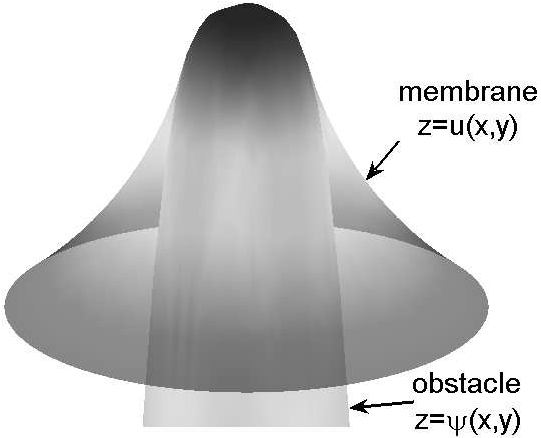
\includegraphics[width=1.1\textwidth]{classicalobs}
\end{center}
\end{column}
\begin{column}{0.65\textwidth}
\begin{center}
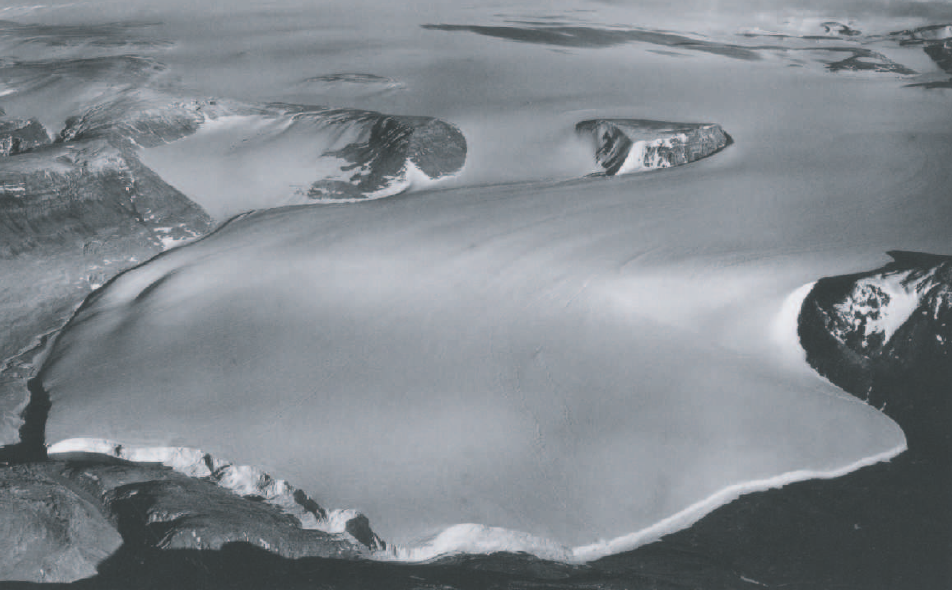
\includegraphics[width=0.8\textwidth]{polaris} \\
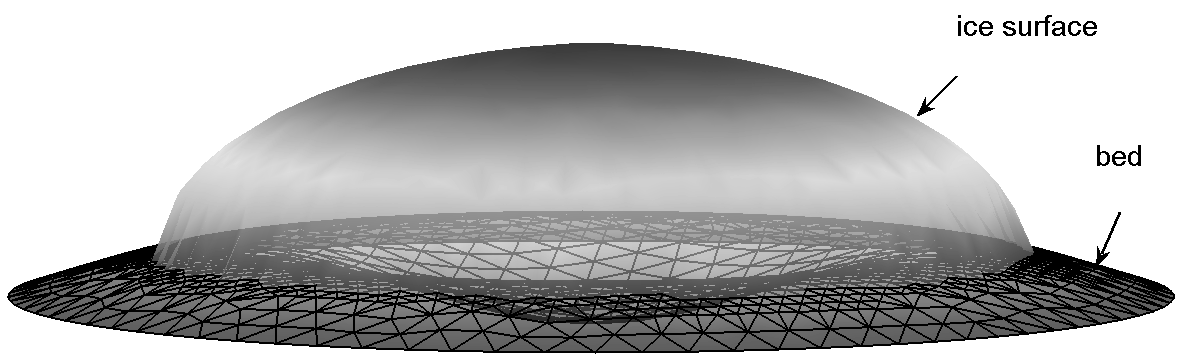
\includegraphics[width=\textwidth]{capnonflatobs}
\end{center}
\end{column}
\end{columns}
\end{frame}


\begin{frame}
  \frametitle{existence and uniqueness for a restricted problem} 

\begin{block}{(easy) theorem}
if $\alpha,\Phi$ were independent of $u$ then the variational inequality is equivalent to:

\begin{equation*}
u \text{ minimizes} \qquad J(v) = \frac{\mu}{p} \int_{\Omega} |\nabla v - \Phi |^p - \int_{\Omega}  \alpha v
\end{equation*}

over $v\in\mathcal{K}$; this admits a unique solution \hfill \scriptsize (Jouvet-Bueler 2012)
\end{block}

\bigskip
\begin{itemize}
\item gives ice sheet existence and uniqueness only if
  \begin{itemize}
  \item[$\circ$]  bedrock is flat ($\Phi = 0$) and
  \item[$\circ$]  mass balance is elevation-independent ($a=a(x,y)$)
  \end{itemize}
\item but otherwise: $\alpha,\Phi$ are not independent of $u$
\end{itemize}
\end{frame}
 

\begin{frame} 
  \frametitle{ existence in the general case } 

\begin{itemize}
\item $p>2$ so $W^{1,p}_0 (\Omega) \hookrightarrow C(\overline{\Omega})$
\item define map $\mathcal{A}:C(\overline{\Omega}) \rightarrow C(\overline{\Omega})$,
which takes $w$ to the unique $u$ solving (over $v\in \mathcal{K}$)
\begin{align*}
\int_{\Omega}   \mu  \left( | \nabla u - \Phi(w) |^{p-2} 
( \nabla u - \Phi(w) )    \right)  \cdot \nabla ( v - u )  
\ge \int_{\Omega} \alpha(w) (  v -  u )
\end{align*}
\end{itemize}

\begin{block}{result}
the map $\mathcal{A}$ admits at least one fixed point \hfill \scriptsize (Jouvet-Bueler 2012)
\end{block}

\vfill
\scriptsize
sketch of proof:
\begin{itemize}
\item $\mathcal{A}$ is continuous and compact
\item the set $\{ w \in C(\overline{\Omega}), \exists \lambda \in [0,1]\, \text{so that} \,w = \lambda \mathcal{A}(w)\}$ is bounded 
\item Schaefer's fixed point theorem
\end{itemize}
\end{frame}


\begin{frame}
  \frametitle{thus: fixed-point iteration on variational inequality} 

\begin{itemize}
\item given bedrock topography $b(x,y)$
\item given mass-balance $a(x,y)$ (steady climate)
\item set $u_0 = 0$
\item do fixed point iterations for $u_{k+1} \in \mathcal{K}$:
\begin{align*}
\int_{\Omega} &\left( \mu |\nabla u_{k+1} - \Phi(u_k)|^{p-2}
(\nabla u_{k+1} - \Phi(u_k) ) \right) \cdot \nabla (v - u_{k+1}) \\
&\qquad\qquad \ge \int_{\Omega} \alpha (v -  u_{k+1})
\end{align*}

\bigskip
\item \emph{computes}: steady state ice sheet shape
\end{itemize}
\end{frame}





\begin{frame}
  \frametitle{SSA for ice streams: an analogy}

\begin{columns}
\begin{column}{0.6\textwidth}
\begin{itemize}
\item ice shelves have zero basal resistance
\item ice streams emerge where basal resistance is sufficiently low

(\emph{top}: Siple coast ice streams)
\item a basal resistance model:
  \begin{itemize}
  \item[$\circ$] ``plastic'' or Coulomb friction 
  \item[$\circ$] distribution of yield stress $\tau_c$
  \end{itemize}
\item ice membrane connects to upstream and/or lateral high friction with viscous stresses (\emph{bottom}: Schoof's slider analogy)
\end{itemize}
\end{column}
\begin{column}{0.4\textwidth}
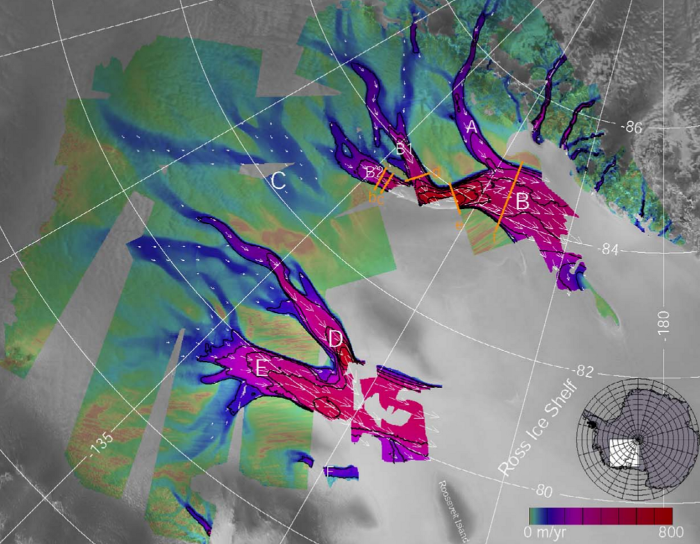
\includegraphics[width=\textwidth]{siple}

\vspace{0.3in}

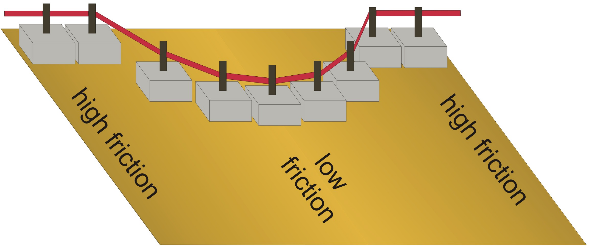
\includegraphics[width=1.1\textwidth]{schoof-sliders}
\end{column}
\end{columns}
\end{frame}


\begin{frame}
  \frametitle{SSA weak formulation}

\begin{itemize}
\item let $q = 1+\frac{1}{n}$ and $B = A^{1-q}$
\item suppose a basal yield stress distribution $\tau_c(x,y)$, zero on ice shelves
\item $2\,\Tnorm{\mathbf{V}}^2 := \sum_{i,j} (\mathbf{D}V_{ij})^2 + \sum_{i} (\mathbf{D}V_{ii})^2$
\item $\mathbf{F}$ denotes lateral force along calving front
\end{itemize}

\begin{block}{definition}
the horizontal velocity $\mathbf{U}\in W^{1,q}(\Omega)$ solves the coulomb friction SSA if it minimizes
\small
\begin{align*}
\mathcal{J}_{\text{SSA}}(\mathbf{V}) &= \int_\Omega \frac{2 B}{q} h \Tnorm{\mathbf{V}}^q + \rho g h \grad s \cdot \mathbf{V} + \tau_c |\mathbf{V}| - \int_{\partial\Omega} \mathbf{F} \cdot \mathbf{V}
\end{align*}
\end{block}

\end{frame}


\begin{frame}
  \frametitle{SSA weak formulation is well-posed}

\bigskip
\begin{block}{Theorem}
if $h\in L^\infty(\Omega)$ with $h\ge h_0>0$, and if $h |\grad s| \in L^{q/(q-1)}(\Omega)$, and if  $\tau_c \in L^{q/(q-1)}(\Omega)$, and as long as there is sufficient total basal resistance,$^\ast$ then the Coulomb friction SSA is well-posed problem for computing the velocity $\mathbf{U}\in W^{1,q}(\Omega)$ \hfill \scriptsize (Schoof, 2006)
\end{block}

\bigskip
\begin{itemize}
\item \emph{note}: because $\mathcal{J}_{\text{SSA}}$ is not differentiable, minimization on last slide is equivalent to a variational inequality but not to a PDE
\end{itemize}

\vfill
\scriptsize $\ast$: To stop the ice sheet from sliding whole into the sea.  There is a precise inequality.
\end{frame}

\begin{frame}
  \frametitle{marine ice sheets}

\begin{itemize}
\item marine ice sheets have all modes of flow
\item full of free boundaries
\item the Antarctic ice sheet is the marine ice sheet
\end{itemize}

\begin{center}
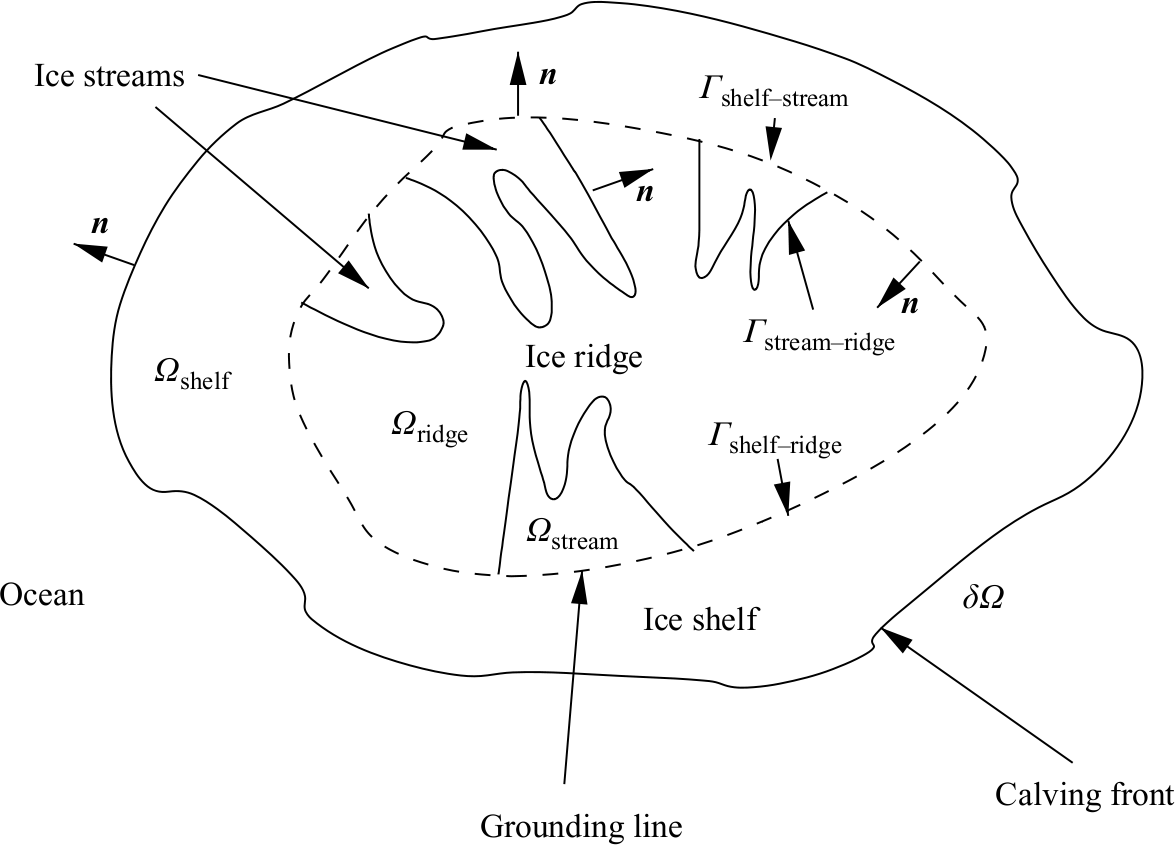
\includegraphics[width=0.7\textwidth]{schoof-planform}

\tiny cartoon from (Schoof, 2006)
\end{center}
\end{frame}







\begin{frame}
  \frametitle{a quality of the SIA variational inequality} 

\begin{itemize}
\item every glaciologist believes this about steady climates:
	$$\text{if } a > 0 \text{ on a sub-domain } R \text{ then } s > b \text{ on } R$$
\item that is:
\begin{center}
 if it snows more than it melts then you get a glacier there
\end{center}
\end{itemize}

\begin{columns}
\begin{column}{0.6\textwidth}
\begin{itemize}
\small
\item uniformly-elliptic variational inequalities, e.g.~the classical obstacle problem,
\begin{align*}
\int_{\Omega}  \nabla u \cdot \nabla (v - u)  \ge  \int_{\Omega} f (v - u),
\end{align*}
for all $v\ge \psi$, do \emph{not} have the analogous property
\end{itemize}
\end{column}
\begin{column}{0.4\textwidth}
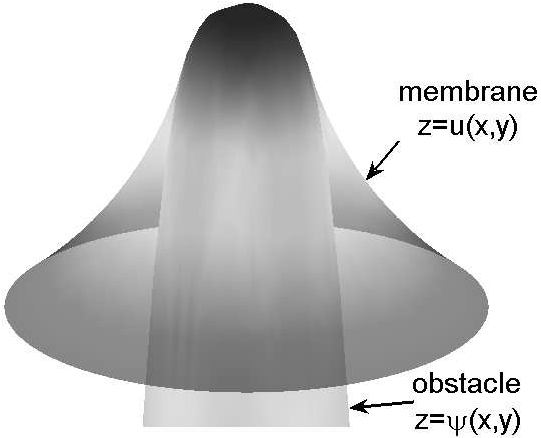
\includegraphics[width=\textwidth]{classicalobs}
\end{column}
\end{columns}
\end{frame}




\end{document}
